\textbf{Photoluminescence} is the emission of light by the excited molecules and/or 
molecule clusters. Here we are intended to observe photon emission from the defects 
within crystalline structures such as diamond and cubic boron nitride. Given that these
materials known to be opaque in visible light range, we are building a \textbf{reflecting 
light microscope}[refhere]. Although wide-field excitation (similar to epifluorescence 
[refhere]) based emission measurements from an ensemble of defects have their own 
importance in characterization, we pursue investigating properties of individual defects/
emitters. This requires our reflecting light microscope to be a \textbf{confocal system}.  

\subsection{Reflecting Light Microscopes Overview}
On typical an upright or inverted microscope, illumination light comes from a direction 
relative to sample surface, while the collection or imaging is done in the opposite direction. 
Therefore in terms of optical components, illumination and imaging sides differ in those
systems. For example in illumination side a special lens called \textbf{Condenser} focuses
the light on to the sample while in the imaging side another special lens called \textbf{
Objective} lens collects the light coming from the sample. These special lenses and the
typical upright and inverted microscope configurations are shown in Figure\ref{fig:CondenserAndObjective}.

\begin{figure}[H]
	\centering
	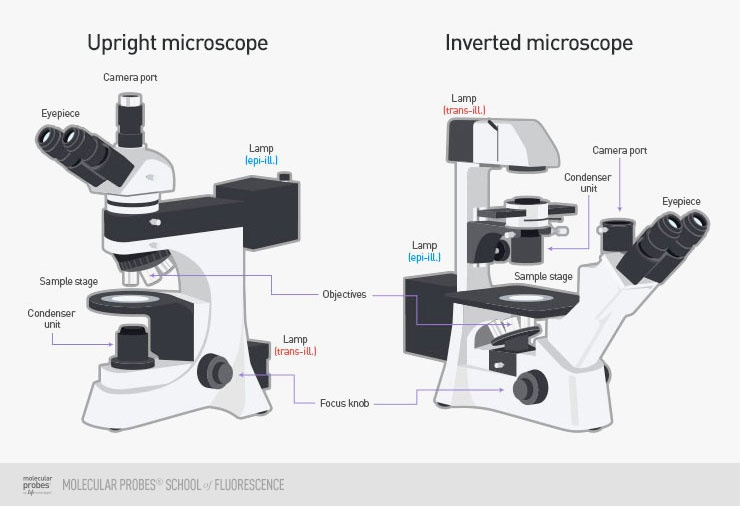
\includegraphics[angle=0,origin=c,width = 1.0\linewidth]{Section_Microscope/Figures/CondenserAndObjective.jpg}
	\caption{A typical upright (\textbf{left}) and an inverted (\textbf{right}) microscope 
		structures indicating the positions of special lenses (\textbf{Condenser and objective}).}
	\label{fig:CondenserAndObjective}
\end{figure}

On the other hand, in a reflecting microscope illumination and imaging are done through the
same optical path or by same optics. As it is shown in Figure\ref{fig:ReflectingMicroscope},
shared optical path allows one (1) additional port for imaging and/or illuminating the sample
on a typical reflecting microscope. This port is very frequently assigned to white-light
(\textbf{bright-field}) imaging through a camera, so it is called the camera port. As a result
any additional illumination and/or imaging on top of the default system, require a custom
design optical system with the ability to finely couple with the existing microscope.

\begin{figure}[H]
	\centering
	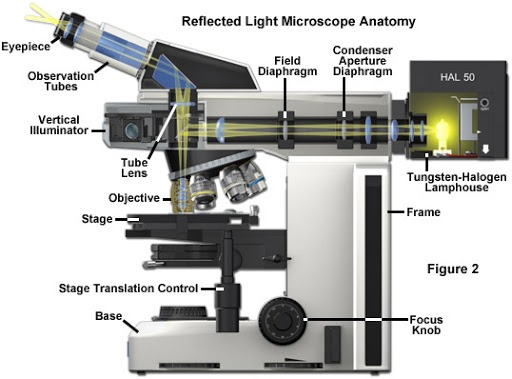
\includegraphics[angle=0,origin=c,width = 1.0\linewidth]{Section_Microscope/Figures/ReflectingMicroscope.jpeg}
	\caption{Schematics of a typical reflecting microscope with light path and internal 
		optical components.}
	\label{fig:ReflectingMicroscope}
\end{figure}

\subsection{Confocal Systems Overview}

\subsection{Our Current PL Setup}
